\documentclass[a4paper]{article}
\usepackage[T1]{fontenc}			% pacchetto per \chapter
\usepackage[italian]{babel}
\usepackage[italian]{isodate}  		% formato delle date in italiano
\usepackage{graphicx}				% gestione delle immagini
\usepackage{amsfonts}
\usepackage{booktabs}				% tabelle di qualità superiore
\usepackage{mathrsfs, amsmath}				% pacchetto matematica
\usepackage{mathtools}				% per sottolineare sotto le equazioni
\usepackage{stmaryrd} 				% per '\llbracket' e '\rrbracket'
\usepackage{amsthm}					% teoremi migliorati
\usepackage{enumitem}				% gestione delle liste
\usepackage{pifont}					% pacchetto con elenchi carini
\usepackage{enumitem}				% pacchetto per elenchi con lettere dell'alfabeto
\usepackage{cancel}					% per cancellare delle espressioni matematiche
\usepackage{listings}				% implementa codice di programmazione
\usepackage{mathalpha}
\usepackage{caption}


\usepackage[x11names]{xcolor}		% pacchetto colori RGB
% Link ipertestuali per l'indice
\usepackage{xcolor}
\usepackage[linkcolor=black, citecolor=blue, urlcolor=cyan]{hyperref}
\hypersetup{
	colorlinks=true
}

% Colour code style
\definecolor{codegreen}{rgb}{0,0.6,0}
\definecolor{codegray}{rgb}{0.5,0.5,0.5}
\definecolor{codepurple}{rgb}{0.58,0,0.82}
\definecolor{backcolour}{rgb}{0.95,0.95,0.92}

\lstdefinestyle{MATLAB}{
	backgroundcolor=\color{backcolour},   
	commentstyle=\color{codegreen},
	keywordstyle=\color{magenta},
	numberstyle=\tiny\color{codegray},
	stringstyle=\color{codepurple},
	basicstyle=\ttfamily\footnotesize,
	breakatwhitespace=false,         
	breaklines=true,                 
	captionpos=b,                    
	keepspaces=true,                 
	numbers=left,                    
	numbersep=5pt,                  
	showspaces=false,                
	showstringspaces=false,
	showtabs=false,                  
	tabsize=2
}
\lstset{style=MATLAB}

%\usepackage{showframe}				% visualizzazione bordi
%\usepackage{showkeys}				% visualizzazione etichetta

\newtheorem{theorem}{\textcolor{Red3}{\underline{Teorema}}}
\newtheorem{lemma}{Lemma}
\renewcommand{\qedsymbol}{QED}
\newcommand{\exec}[1]{\llbracket #1\:\rrbracket}
\newcommand{\dquotes}[1]{``#1''}
\newcommand{\longline}{\noindent\rule{\textwidth}{0.4pt}}

\begin{document}
	\author{Università degli Studi di Verona}
	\title{Soluzione - Esame di Elaborazione di segnali e immagini}
	\date{{\Large 01 Febbraio 2021}}
	\maketitle
	
	\section{Soluzione Esercizio (10 punti)}
	
	Si descrive in modo analitico il segnale nel dominio delle frequenze ricordando che la funzione $\mathrm{sinc}$ rappresenta la box e l'esponenziale il suo shift:
	\begin{equation*}
		\begin{array}{lll}
			\text{Dominio nel tempo} 		& \longrightarrow & g\left(t\right) = 40\mathrm{sinc}\left(20t\right) + 15\mathrm{sinc}\left(30t\right) e^{-j 2 \pi 45 t} + 15\mathrm{sinc}\left(30t\right) e^{j 2 \pi 45 t} \\
			\\
			\text{Dominio nelle frequenze} 	& \longrightarrow & G\left(\mu\right) = 2\Pi\left(\dfrac{\mu}{20}\right) + \dfrac{1}{2}\Pi\left(\dfrac{\mu - 45}{30}\right) + \dfrac{1}{2}\Pi\left(\dfrac{\mu + 45}{30}\right)
		\end{array}
	\end{equation*}
	Graficamente il segnale è composto da tre box, una centrata nell'origine e due all'estremo shiftate nel tempo.
	\begin{figure}[!htp]
		\centering
		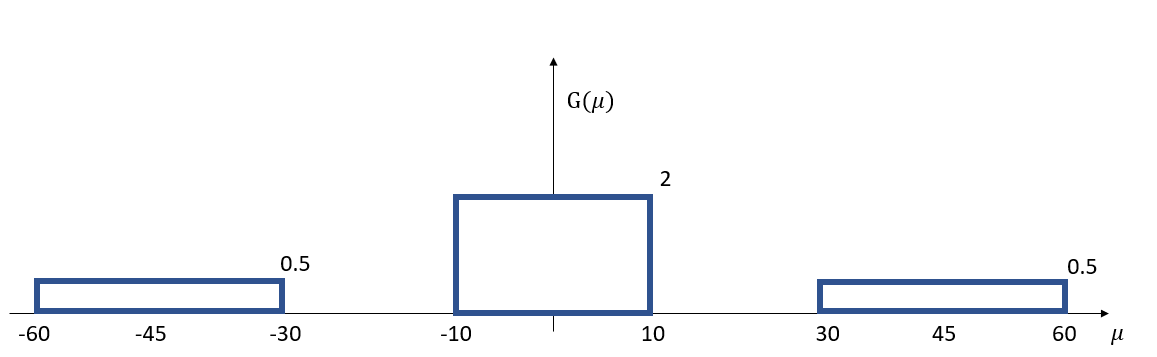
\includegraphics[width=\textwidth]{img/fig_1.png}
		\caption*{Rappresentazione grafica del segnale $G\left(\mu\right)$ nel dominio delle frequenze.}
	\end{figure}\newpage

	\subsection*{\textcolor{Green4}{\emph{\underline{Passa basso ideale $\boldsymbol{a\left(t\right)}$}}}}
	
	Un filtro passa basso ideale ha l'obbiettivo di tagliare le frequenze alte e lasciare le basse. Esso viene rappresentato come una box nel dominio delle frequenze e la funzione $\mathrm{sinc}$ nel dominio del tempo. Quindi, il filtro analiticamente è:
	\begin{equation*}
		\begin{array}{lll}
			\text{Dominio nel tempo} 		& \longrightarrow & 30\mathrm{sinc}\left(30t\right) \\
			\\
			\text{Dominio nelle frequenze} 	& \longrightarrow & \Pi\left(\dfrac{\mu}{30}\right)
		\end{array}
	\end{equation*}
	L'applicazione del filtro passa basso ideale nel dominio del tempo è una convoluzione. Quindi, per definizione, nel dominio delle frequenze il segnale da filtrare e il filtro dovranno essere moltiplicati. Analiticamente nel dominio delle frequenze si ha:
	\begin{equation*}
		A\left(\mu\right) = G\left(\mu\right) \cdot \Pi\left(\dfrac{\mu}{30}\right) = 2\Pi\left(\dfrac{\mu}{20}\right)
	\end{equation*}
	Analogamente, nel dominio del tempo si ha:
	\begin{equation*}
		a\left(t\right) = g\left(t\right) * 30\mathrm{sinc}\left(30t\right) = 40\mathrm{sinc}\left(20t\right)
	\end{equation*}
	\begin{figure}[!htp]
		\centering
		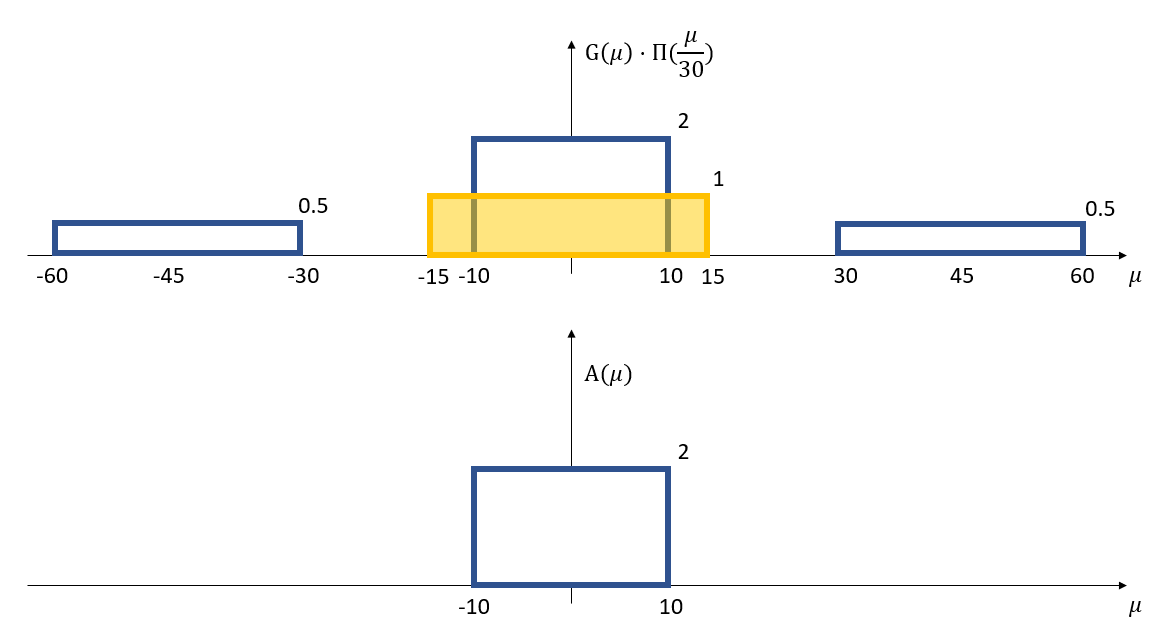
\includegraphics[width=\textwidth]{img/fig_2.png}
		\caption*{Rappresentazione grafica del segnale $A\left(\mu\right)$.}
	\end{figure}\newpage

	\subsection*{\textcolor{Green4}{\emph{\underline{Campionatore $\boldsymbol{b\left(t\right)}$}}}}
	
	Il campionatore consente di riprodurre il segnale all'infinito. Questo è possibile poiché il segnale viene moltiplicato per un treno di impulsi. Infatti, il segnale nel dominio del tempo corrisponde ad una moltiplicazione (treno di impulsi), mentre nel dominio delle frequenze si ha una convoluzione. Si sviluppa analiticamente quest'ultima:
	\begin{equation*}
		\begin{array}{lll}
			B\left(\mu\right) & = & A\left(\mu\right) * 20\displaystyle\sum_{n} \delta\left(\mu - 20n\right) \\
			\\
			& = & \displaystyle\int_{-\infty}^{\infty} A\left(\tau\right) \cdot 20\displaystyle\sum_{n} \delta\left(\mu - 20n - \tau\right) \\
			\\
			& = & 20 \cdot \displaystyle\int_{-\infty}^{\infty} A\left(\tau\right) \cdot \displaystyle\sum_{n} \delta\left(\mu - 20n - \tau\right) \\
			\\
			& \downarrow & \text{Proprietà di setacciamento} \\
			\\
			& = & 20 \cdot \displaystyle\sum_{n} A\left(\mu - 20n\right)
		\end{array}
	\end{equation*}
	Il dominio nel tempo è il seguente:
	\begin{equation*}
		b\left(t\right) = a\left(t\right) \cdot \displaystyle\sum_{n} \delta\left(\dfrac{t - n}{20}\right)
	\end{equation*}
	Dal grafico si nota che non si presenta aliasing ma appaiamento. Il segnale dunque è costante.
	\begin{figure}[!htp]
		\centering
		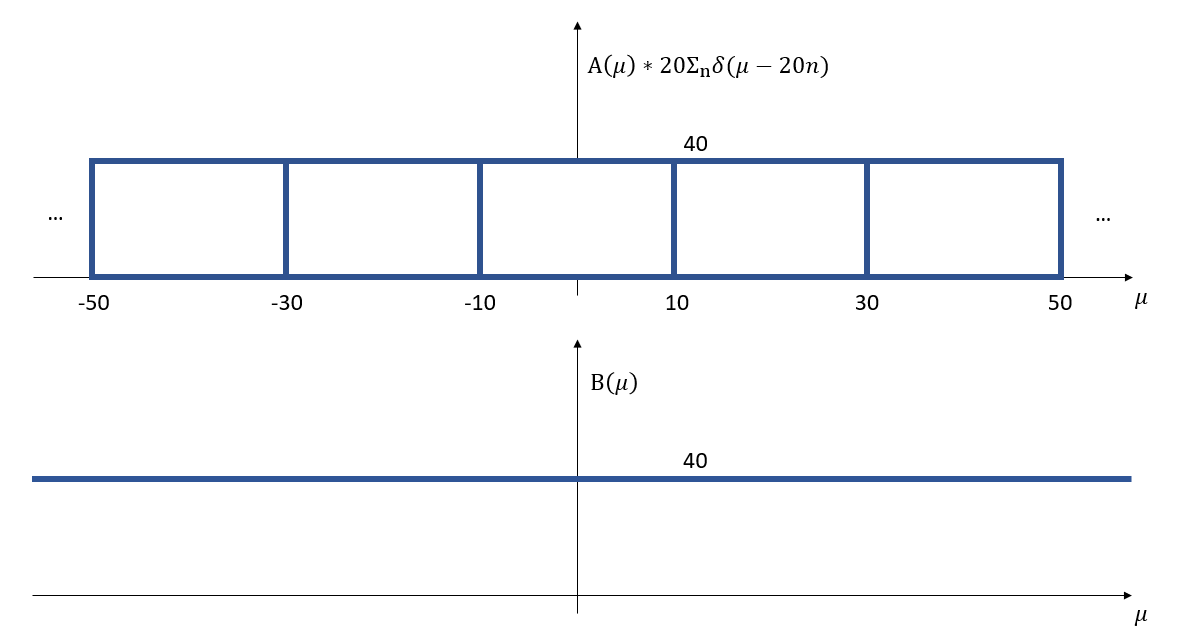
\includegraphics[width=\textwidth]{img/fig_3.png}
		\caption*{Rappresentazione grafica del segnale $B\left(\mu\right)$.}
	\end{figure}\newpage

	\subsection*{\textcolor{Green4}{\emph{\underline{Passa basso ideale $\boldsymbol{c\left(t\right)}$}}}}
	
	Un filtro passa basso ideale ha l'obbiettivo di tagliare le frequenze alte e lasciare le basse. Esso viene rappresentato come una box nel dominio delle frequenze e la funzione $\mathrm{sinc}$ nel dominio del tempo. Quindi, il filtro analiticamente è:
	\begin{equation*}
		\begin{array}{lll}
			\text{Dominio nel tempo} 		& \longrightarrow & 100\mathrm{sinc}\left(100t\right) \\
			\\
			\text{Dominio nelle frequenze} 	& \longrightarrow & \Pi\left(\dfrac{\mu}{100}\right)
		\end{array}
	\end{equation*}
	L'applicazione del filtro passa basso ideale nel dominio del tempo è una convoluzione. Quindi, per definizione, nel dominio delle frequenze il segnale da filtrare e il filtro dovranno essere moltiplicati. Analiticamente nel dominio delle frequenze si ha:
	\begin{equation*}
		A\left(\mu\right) = B\left(\mu\right) \cdot \Pi\left(\dfrac{\mu}{100}\right) = 40\Pi\left(\dfrac{\mu}{100}\right)
	\end{equation*}
	Analogamente, nel dominio del tempo si ha:
	\begin{equation*}
		a\left(t\right) = b\left(t\right) * 100\mathrm{sinc}\left(100t\right) = 4000\mathrm{sinc}\left(100t\right)
	\end{equation*}
	\begin{figure}[!htp]
		\centering
		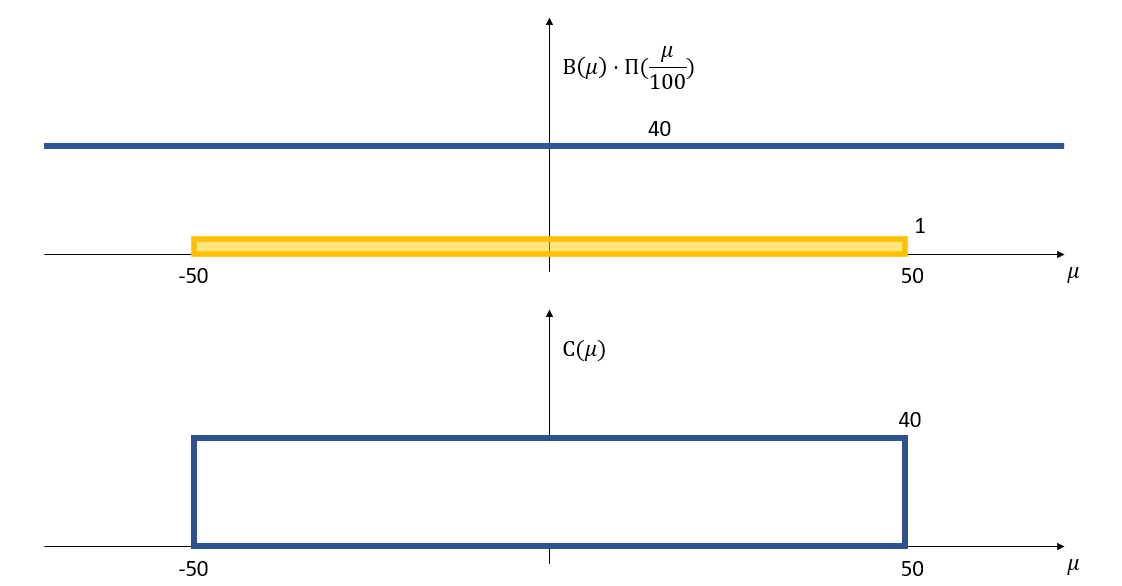
\includegraphics[width=\textwidth]{img/fig_4.png}
		\caption*{Rappresentazione grafica del segnale $C\left(\mu\right)$.}
	\end{figure}\newpage

	\section{Soluzione Esercizio (9 punti)}
	
	I due segnali, analiticamente parlando, nel dominio delle frequenze sono:
	\begin{equation*}
		\begin{array}{lll}
			X\left(\mu\right) & = & \Pi\left(\dfrac{\mu - 0.25}{0.5}\right) \\
			\\
			H\left(\mu\right) & = & 2\Pi\left(\dfrac{\mu - 0.5}{1}\right)
		\end{array}
	\end{equation*}
	Graficamente la convoluzione è:
	\begin{figure}[!htp]
		\centering
		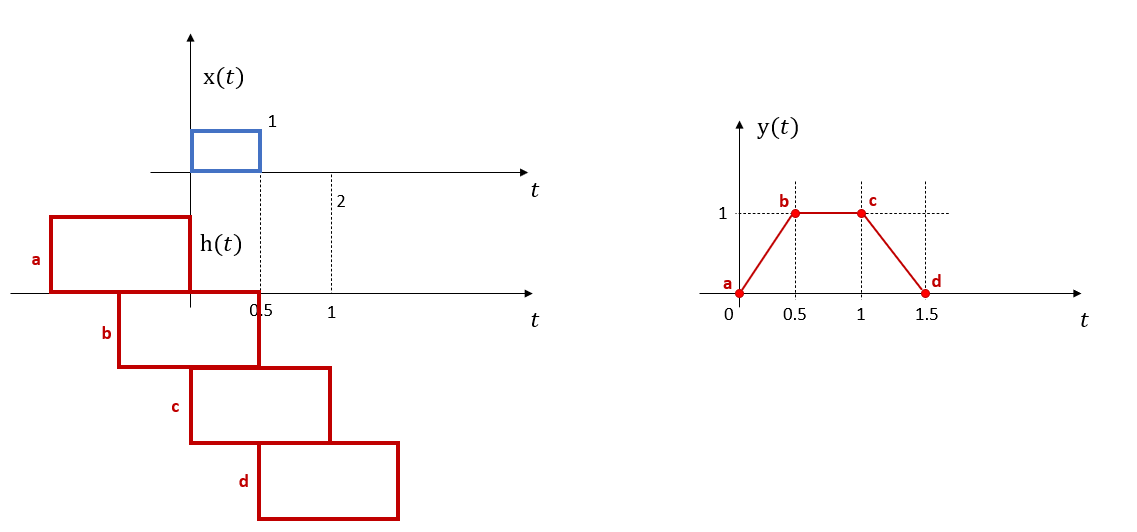
\includegraphics[width=\textwidth]{img/fig_5.png}
		\caption*{Rappresentazione grafica della convoluzione.}
	\end{figure}
	
	\noindent
	Assumendo che negli estremi $h\left(t\right)$ valga zero e quindi con $t < 0$ non vi è intersezione e il segnale $y$ non esiste, si descrive lo sviluppo della convoluzione:
	\begin{enumerate}[label=\alph*)]
		\item $t = 0$, vi è intersezione con l'inizio della box, ma il prodotto tra i segnali è uguale a zero. Quindi, l'integrale vale zero: $y\left(0\right) = 0$;
		
		\item $t = 0.5$, vi è intersezione e il prodotto tra i segnali è una box di ampiezza $2$ e base $0.5$. Quindi, l'integrale vale uno: $y\left(0.5\right) = 1$;
		
		\item $t = 1$, vi è intersezione e il prodotto tra i segnali è una box di ampiezza $2$ e base $0.5$. Quindi, l'integrale vale uno: $y\left(1\right) = 1$;
		
		\item $t = 1.5$, vi è intersezione con la fine della box, ma il prodotto tra i segnali è uguale a zero. Quindi, l'integrale vale zero: $y\left(1.5\right) = 0$.
	\end{enumerate}
	Con $t > 1.5$ non vi è intersezione e il segnale $y$ non esiste.\newpage
	
	\section{Soluzione Esercizio (6 punti)}
	
	\subsection*{\textcolor{Green4}{\emph{\underline{Risposta domanda a}}}}
	
	Un filtro passa basso ideale è un'operazione applicata ai segnali con l'obbiettivo di rimuovere le alte frequenze e di lasciare intatte solamente quelle basse all'interno del \dquotes{range} del filtro. La parola ideale deriva dal fatto che la frequenza di taglio (\emph{cutoff}) di questo filtro non è elettronicamente possibile. Infatti, prendendo il suo dominio nelle frequenze, esso corrisponde ad una box rettangolare con delle salite e delle discese troppo repentine.\newline
	
	\noindent
	Nel \underline{dominio del tempo} si rappresenta tramite la funzione $\mathrm{sinc}$. Ad un segnale in entrata, si applica tale filtro eseguendo una convoluzione tra i due segnali.\newline
	
	\noindent	
	Al contrario, nel \underline{dominio delle frequenze} si rappresenta tramite la funzione $\Pi$. Ad un segnale in entrata, si applica tale filtro eseguendo una moltiplicazione tra i due segnali.\newline
	
	\noindent
	Gli effetti nel dominio duale sono l'eliminazione di tutti i segnali fuori dalle frequenze del filtro. Mentre per quanto riguarda l'ampiezza (altezza), essa rimane invariata.\newpage
	
	\subsection*{\textcolor{Green4}{\emph{\underline{Risposta domanda b}}}}
	
	Il rumore nelle immagini è un disturbo dell'immagine introdotto dal sistema di acquisizione (e.g. fotocamera digitale di un dispositivo elettronico come il cellulare) o dal mezzo di propagazione che ne degrada la qualità (e.g. invio di immagini, non come file, con l'app di messaggistica WhatsApp e Telegram).\newline
	
	\noindent
	I \textbf{tipi di rumore} visti a lezione sono due:
	\begin{itemize}
		\item \textbf{Gaussiano additivo bianco}. Esso è un processo stocastico, quindi una variabile aleatoria che acquisisce valori casuali nel tempo o nello spazio con alcune caratteristiche come la non periodicità nel tempo o nello spazio.\newline
		In altre parole, il gaussiano additivo bianco viene generato da una distribuzione gaussiana. Un esempio:
		\begin{figure}[!htp]
			\centering
			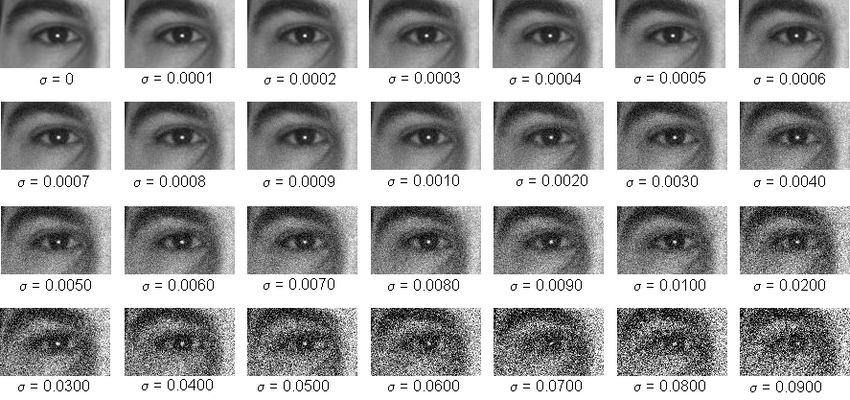
\includegraphics[width=\textwidth]{img/fig_6.png}
		\end{figure}
		
		\item \textbf{Rumore impulsivo}. Esso è causato da alterazioni brusche del segnale. Queste variazioni sono parametrizzate da un fattore (una percentuale) che rappresenta la densità con cui esso si localizza su pixel dell'immagine. Quindi, maggiore è il valore di intensità, maggiore saranno il numero di pixel affetti. Un esempio di filtro è il classico disturbo sale e pepe (\emph{salt-and-pepper noise}).\newline
		In altre parole, il rumore impulsivo viene generato da una distribuzione bernoulliana. Un esempio:
		\begin{figure}[!htp]
			\centering
			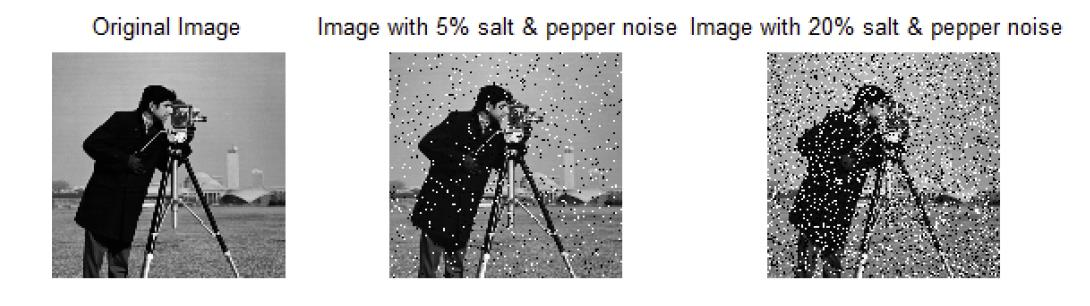
\includegraphics[width=\textwidth]{img/fig_7.png}
		\end{figure}
	\end{itemize}\newpage
	
	\noindent
	Per \textbf{risolvere il rumore} è necessario prima capire quale dei due elencati è. Dopodiché è possibile decidere se rimuoverlo completamente o attenuarlo.\newline
	
	\noindent
	Per \textbf{attenuare} il rumore si può utilizzare un'operazione puntuale (operatore che prende in input un pixel e con determinate operazioni ne cambia il valore e lo restituisce come output) chiamata \textbf{\emph{clamping}}. Esso limita l'intensità in un range definito e solitamente viene utilizzato quando i pixel di rumore sono molto chiari o molto scuri. Si tiene a precisare nuovamente che questa operazione \underline{non} risolvere il rumore, ma lo attenua.\newline
	
	\noindent
	Per quanto riguarda il \textbf{rumore Gaussiano additivo bianco}, esso è possibile rimuoverlo tramite il filtro media oppure ridurlo moltissimo con il filtro gaussiano:
	\begin{itemize}
		\item \textbf{Filtro di media} è un filtraggio lineare e si applica tramite la convoluzione dell'immagine con la maschera media la quale ha alcune caratteristiche:
		\begin{itemize}
			\item Dimensioni $K\times K$ con $K$ dispari;
			\item I suoi coefficienti sono tutti uguali e di pattern $\frac{1}{K^{2}}$;
		\end{itemize}
		La maschera viene applicata ad ogni locazione dell'immagine. Quindi, l'operazione non è altro che una combinazione lineare convessa. Ovvero, la somma dei livelli di grigio dell'immagine originale e di quella processata sono uguali (a meno di padding).\newline
		\textcolor{Green4}{\textbf{Pro:}} rimozione completa del rumore.\newline
		\textcolor{Red3}{\textbf{Contro:}} operazione di \emph{smoothing} molto forte, i dettagli vengono diminuiti, quindi è necessario applicare un'operazione di \emph{sharpening} dopo l'operazione di filtraggio di media.
		
		\item \textbf{Filtro gaussiano} è un filtraggio simile a quello di media ma che ha come valore di input la variabile $\sigma$ che rappresenta la forza dell'operazione. Maggiore sarà la forza, maggiore sarà lo \emph{smoothing}. La differenza sostanziale è che questo filtro utilizza una media pesata con pesi più alti al centro della maschera.\newline
		\textcolor{Green4}{\textbf{Pro:}} con uno \emph{smoothing} più leggero, i dettagli non vengono diminuiti bruscamente. Quindi, si preserva meglio la struttura.\newline
		\textcolor{Red3}{\textbf{Contro:}} il rumore non viene tolto del tutto.
	\end{itemize}\:\newline

	\noindent
	Infine, per il \textbf{rumore impulsivo} esiste il \textbf{filtro mediano} che consente di rimuovere il rumore. L'operazione è banale e viene eseguita tramite un algoritmo. Si prendono i valori della matrice, si mettono in ordine crescente e si calcola la relativa mediana.\newpage
	
	\subsection*{\textcolor{Green4}{\emph{\underline{Risposta domanda c}}}}
	
	Analiticamente parlando, il rumore può essere misurato tramite un valore particolare. Si dice che la \textbf{quantità di rumore} viene stimata con la misura di \emph{Signal to Noise Ratio} (\emph{SNR}). Esistono molte versioni, ma la più utilizzata è la \emph{\textbf{mean square}}:
	\begin{equation*}
		SNR_{ms} = \dfrac{
			\displaystyle\sum_{n=1}^{N}\sum_{m=1}^{M} \tilde{f}\left(n,m\right)^{2}
		}{
			\displaystyle\sum_{n=1}^{N}\sum_{m=1}^{M} \left[\tilde{f}\left(n,m\right) - f\left(n,m\right)\right]^{2}
		}
	\end{equation*}
	Esiste una forma alternativa, forse anche più leggibile. Essa si basa sul fatto che il SNR può essere stimato grazie alla varianza $\sigma^{2}_{n}$, o alla deviazione standard $\sigma_{n}$:
	\begin{equation*}
		SNR = \dfrac{\sigma_{s}}{\sigma_{n}}
	\end{equation*}
	Dove $\sigma_{s}$ è la deviazione standard del segnale e $\sigma_{n}$ è la deviazione standard dell'immagine affetta da rumore. Da questo si capisce il motivo per cui spesso si utilizzano immagini ad alto contrasto, ovvero che la deviazione standard $\sigma_{s}$ risulta maggiore.
\end{document}